\section{A Normal Profile Walkthrough}
\label{sec:design}
\label{sec:normal-profile}

Consider a profile $\pi$ with a nonresident weight dependency. The following
walkthrough composes protocol roles; it is not a claim that every TP1 runner
uses the general registry. It connects the resource model to the algorithms
and to the observables evaluated in Section~\ref{sec:evaluation}.

\paragraph{Plan and admit.}
The adapter binds source descriptors, representation, placement, and workspace.
The destination authority supplies the actual reservation and reuse generation.
The resulting $P=(K,\boldsymbol q,\boldsymbol\ell)$ is frozen before hard
admission. Equation~\ref{eq:admission} is a necessary covered-domain check,
not complete admission or a sum of heterogeneous budgets. The stage also
passes authority, compatibility, intrinsic-capacity, and execution-reserve
checks in Section~\ref{sec:scope}. An impossible stage is rejected; only
otherwise admissible demand blocked by current occupancy waits. Before preparation can submit physical
work, the owner records provisional state and cleanup intent in journal $J$.

\paragraph{Read, transfer, and install.}
A new load admits read/staging claims and submits once. Exact read completion
returns named read custody. On read success, the owner then explicitly
releases held ReadSlot and StorageReadBytes credits while retaining the
pinned buffer and PinnedHostBytes charge for upload. Custody return alone
is not that credit discharge. Upload needs
its own admission and retained fence; its completion ends DMA custody but not
destination ownership. Installation admits its own claims. Replacement also
needs evidence that old consumers have stopped using the old binding. An
ambiguous submission retains its ticket, allocations, and claims even when no
public handle is returned.

\paragraph{Publish and consume.}
Install success is validated against operation, key, stage, bytes, and both
generations. Publication preflight checks the actual binding and replacement
rules. Ready permits resident-grant transfer and exact waiter resolution;
Blocked waits for replacement leases/custody to end; Rejected preserves the
original journal, grants, and physical binding for terminal cleanup instead
of publishing or refunding residency. Only Ready retires the load operation
by transferring its resident grant. This is not eviction: resident bytes
remain charged. A consumer revalidates its dependency and lease epochs and
obtains resume admission before executing. A compatible resident hit skips
materialization; a compatible in-flight load can be joined only on paths that
implement sharing.

\paragraph{Bounded next-expert scheduling.}
On the concrete routed-expert path, the owner first uploads the current
expert and retires its temporary host payload aliases. It can then submit one
read for the next selected, nonresident expert before submitting current
compute. A read-only residency hint neither pins that next expert nor changes
cache replacement order. Blocking uses the same worker and waits at demand
instead. This split is a scheduling candidate, not a measured GPU overlap or
an asynchronous forward API (Algorithm~\ref{alg:bounded-lookahead}).

\paragraph{End and retire.}
Consumer completion returns only the custody discharged by its adapter.
Ending/publication and post-ending cleanup are separate phases. Prepared-KV
owners require exact install acknowledgments before logical publication and
retirement acknowledgments before displaced pages are reused. Independent
cache pins and persistent state survive request completion. Cancellation
changes the caller outcome, not these end conditions; Unknown may retain
capacity indefinitely.

\begin{figure}[tbp]
\centering
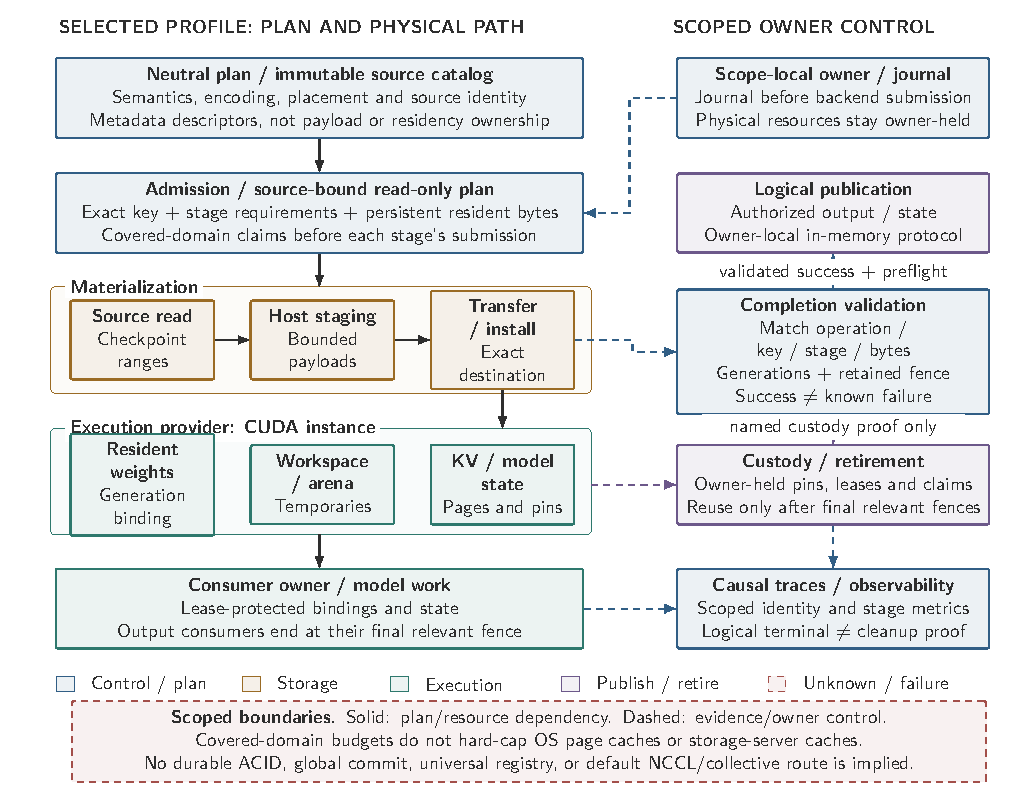
\includegraphics[width=\linewidth]{figures/architecture.pdf}
\caption{Conceptual, profile-scoped architecture. The shared palette uses blue
for control/planning/validation, ochre for storage/materialization, teal for
execution/provider resources, violet for publication/custody/retirement, and
brick for Unknown/failure. Named nodes and labeled swatches carry the meaning
independently of color. Solid arrows denote dependencies; dashed arrows name
evidence or owner-control gates. Source planning and covered-domain admission
precede materialization; providers retain physical resources. CUDA is one
provider instance. No universal registry, OS-cache hard cap, durable/cross-rank
ACID, or default NCCL/device-collective route is implied.}
\label{fig:architecture}
\end{figure}

The walkthrough supplies three different evidence gates: startup final-claim
completion, materialization producer/replacement completion, and consumer/
ending completion. None substitutes for another. The experiment should record
those transitions alongside complete-output quality, physical memory samples,
and request I/O. The arrows in Figure~\ref{fig:architecture} are conceptual
dependencies, not measured hardware overlap.

\section{Design Invariants}
\label{sec:invariants}

These are intended contracts for the implemented boundaries, not completed
formal verification or independently measured properties of every profile.

\paragraph{I1: bounded, uniquely owned claims.}
Admitted claims must preserve $U_a+c_a\leq b_a$, together with the demand
policy and authority checks; this inequality alone is not admission. For each accounting domain, the
intended semantic partition is
\begin{equation}
\begin{aligned}
 b_a&=F_a+R_a+I_a+L_a+T_a,\\
 U_a&=R_a+I_a+L_a+T_a,\qquad F_a=b_a-U_a .
\end{aligned}
\label{eq:credit-conservation}
\end{equation}
Each claim occupies exactly one class: free, reserved, provider-in-flight,
live, or retained. Different claims of one operation can occupy different
classes. Unknown is classified in $T_a$, not charged again as $I_a+T_a$.
Returning provider custody does not necessarily decrease $U_a$: an explicit
release or ownership transfer is separate. The broker records capacity,
occupancy, authenticated owner, and a submitted bit, not five literal bucket
fields. Equation~\ref{eq:credit-conservation} is an intended invariant;
the serving read ledger does not independently measure this general partition
under faults. RQ4 separates observed owner-local closure from the missing
integrated fault and physical-release evidence.

\paragraph{I2: exact evidence before mutation.}
A completion must match $o$, $K$, submitted stage, $g_s$, $g_x$, and
outcome-specific bytes. Success requires the full expected amount; partial
failure is not readiness. Identity-stale, retired, unowned, wrong-stage,
or generation-mismatched events are rejected before mutation and cannot
release a newer generation's grants. In contrast, a matching completion whose
validated \texttt{CompletionOutcome::Stale} reports non-success ends the
named stage according to its proof and selects terminal cleanup; it is not
an identity rejection and does not authorize publication.
Waiter/request/dependency epochs and mapping epochs have different scopes;
a wake notification is not validation of any of them.

\paragraph{I3: custody follows physical work.}
Every outstanding physical reference is required to remain reachable from an
authoritative owner, including on submission, notification, preparation, or cleanup errors.
Read return, upload-fence return, resident transfer, and consumer retirement
close different obligations. An address descriptor is not allocation ownership
or a completion certificate. A read snapshot is not mutation authority.

\paragraph{I4: publication and reuse have different proofs.}
Producer success makes a candidate ready. Publication additionally checks the
actual binding and authorization; old-consumer quiescence and retirement
permit replacement reuse. Typed committed-KV sources and append witnesses are
revalidated against the current page authority, and zero-reference pages are
reused only after retirement confirmation. Several participant ACKs establish
this scoped lifecycle order, not arbitrary distributed atomic commit.

\paragraph{I5: terminal demand does not erase obligations.}
Owner-accepted cancellation detaches only its demand, preserving other
waiters and persistent owners. An unsubmitted shared load is preserved under
its remaining authority or handed off with acknowledgment, never discarded
because one demand ended. Provider cancellation acceptance is recorded once
per exact operation/stage/generation; it is not a quiescence certificate. It cannot reverse an irreversible install/publish intent. Pending
cleanup polls the original identity and arguments without redispatch. Unknown
retains physical payload and credits and preserves applicable owner poison or
quarantine. A matching later registry completion may close a named stage; it
cannot heal a separately poisoned physical owner. No general in-place reset/
replay or unconditional eventual reclamation is asserted.

\begin{figure}[tbp]
\centering
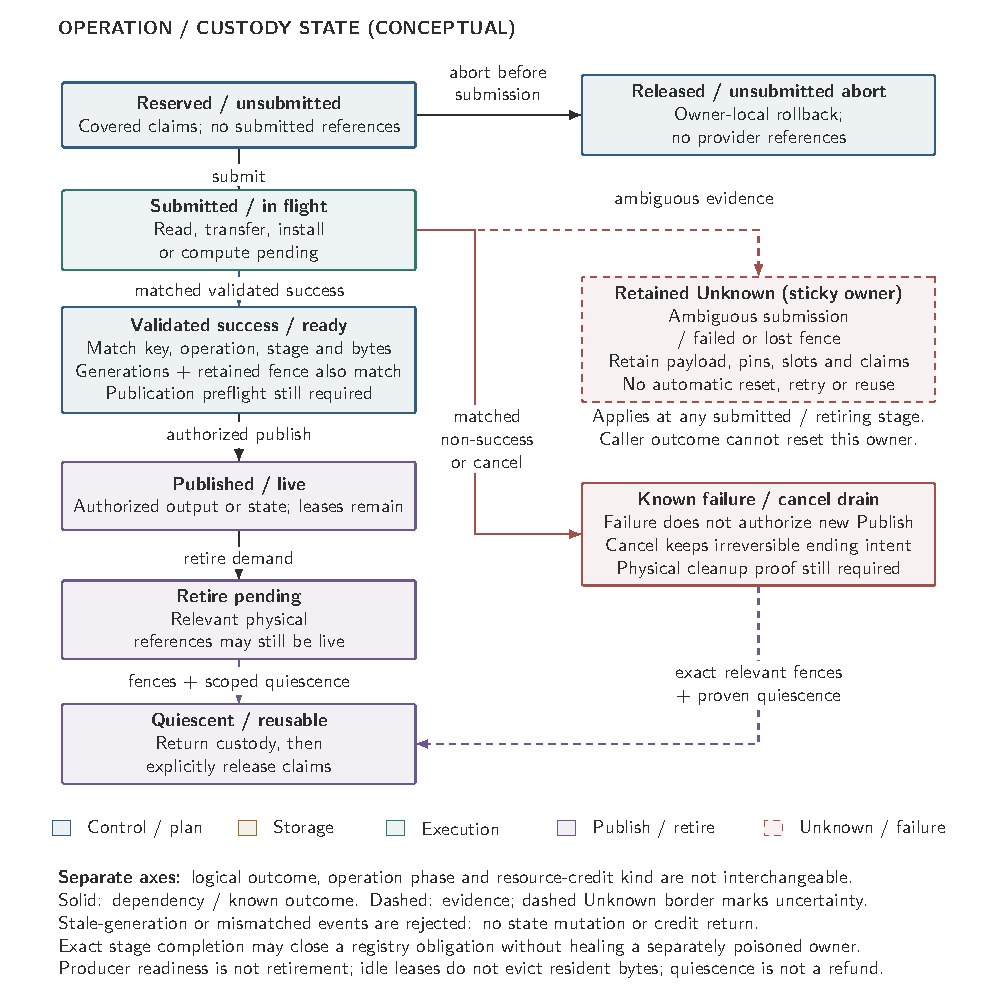
\includegraphics[width=\linewidth]{figures/operation-state.pdf}
\caption{Conceptual operation/custody states, not one Rust enum. Labeled roles
retain the shared blue planning/validation, ochre storage, teal execution,
violet publication/retirement, and brick Unknown/failure palette. Only exact
validated success plus publication preflight authorize new publication.
Known non-success drains the named stage, not readiness; cancellation keeps
irreversible ending intent. Dashed-border physical-owner Unknown retains
payload, pins, slots, and claims and has no automatic recovery/reuse edge.
Closing a matching registry-stage obligation does not heal a separately
poisoned owner. Logical outcomes and charged resources are separate axes.}
\label{fig:operation-state}
\end{figure}

The testable consequences are no stale publication, no duplicate dispatch,
no premature slab/page reuse, and retained capacity when proof is missing.
RQ1 checks bounded completion, RQ2 checks the load demand, RQ3 checks progress
and physical intervals, and RQ4 checks these invariants under faults. A process
exit or idle sample does not independently prove any final owner ledger.

\section{Lifecycle and Bounded Scheduling Algorithms}
\label{sec:algorithms}

The pseudocode names protocol roles and abstract result classes, not new
provider APIs. Its records and journal persist across calls. \textsc{AdmitStage}
validates intrinsic feasibility, canonical claims, authority, compatibility,
and demand/reserve policy before acquiring that stage's grants. An added
claim $c_a>b_a^{\mathrm{eff}}(\delta)$ is intrinsically impossible under that
policy; an otherwise feasible claim blocked by current
$U_a+c_a>b_a^{\mathrm{eff}}(\delta)$ waits. The authoritative owner rechecks
capacity on acquisition, without implying a cross-owner atomic reservation. Rejected
means no further dispatch under the unchanged plan; Wait preserves already
held custody and arms a budget/owner-progress revisit. \textsc{RetainCleanup}
records the primary reason and original payload, then selects the cleanup
protocol in Algorithm~\ref{alg:terminal-custody}; it does not recreate a ticket
or discard other demand. Publication Rejected is the abstract class for
preflight validation/conflict errors, distinct from a live-custody Blocked
result. Rejection after install does not undo the physical installation.
The owner journal records applied custody returns and releases so later
cleanup advances only residual obligations, without applying a return twice.
Cleanup selection is latched: subsequent calls cannot restart normal dispatch
or replace the primary failure reason. Pending/Idle requires a positively
known original pollable obligation; otherwise its custody is Unknown and
retained. Unknown follows cleanup without clearing physical-owner poison.

\begin{algorithm}[tbp]
\caption{Progress one exact materialization operation}
\label{alg:normal-materialization}
\fontsize{9}{9.4}\selectfont
\begin{algorithmic}[1]
\REQUIRE $P:\mathsf{Plan}$, $v:\mathsf{Provider}$, $\mathcal L:\mathsf{Ledger}$,
         $\delta:\mathsf{Demand}$, $J:\mathsf{Journal}$
\ENSURE $h:\{\mathsf{Ready},\mathsf{Pending},\mathsf{Terminal}\}$, $o:\mathsf{LoadRecord}$; residual custody stays reachable
\STATE \textbf{State:} persistent $o:\mathsf{LoadRecord}$; $s:\mathsf{Stage}$;
       $e:\mathsf{Evidence}$; $p:\mathsf{PublicationResult}$;
       $\alpha:\mathsf{AdmissionResult}$
\STATE \textbf{Preconditions:} frozen plan, exact destination, authoritative
       journal; residency/sharing checked
\IF{cleanup is selected or $o$ has retained Unknown}
  \STATE preserve $J,o$; continue only Algorithm~\ref{alg:terminal-custody}
  \RETURN $(\mathsf{Terminal},o)$
\ENDIF
\WHILE{$o.\mathit{phase}\ne\mathsf{Resident}$}
  \IF{$o.\mathit{phase}=\mathsf{Installed}$}
    \STATE \textbf{Publication:} $p\gets\operatorname{Preflight}(o)$
    \IF{$p=\mathsf{Ready}$}
      \STATE publish exact binding; transfer resident grant
      \STATE resolve exact waiters; retire once; $o.\mathit{phase}\gets\mathsf{Resident}$
    \ELSIF{$p=\mathsf{Blocked}$}
      \STATE retain $J,o$; arm replacement-custody revisit
      \RETURN $(\mathsf{Pending},o)$
    \ELSIF{$p=\mathsf{Rejected}$}
      \STATE $\operatorname{RetainCleanup}(J,o,p)$; \algorithmicreturn $(\mathsf{Terminal},o)$
    \ENDIF
  \ELSE
    \STATE $s\gets o.\mathit{stage}$
    \IF{stage $s$ is not submitted}
      \STATE \textbf{Admission:} validate/canonicalize units, overflow, authority,
      \STATE source/placement/backend compatibility, and demand policy
      \IF{validation fails or $\exists a: c_a>b_a^{\mathrm{eff}}(\delta)$}
        \STATE $\alpha\gets\mathsf{Rejected}$ with invalid-plan/intrinsic-capacity reason
        \STATE $\operatorname{RetainCleanup}(J,o,\alpha)$; \algorithmicreturn $(\mathsf{Terminal},o)$
      \ELSIF{$\exists a: U_a+c_a>b_a^{\mathrm{eff}}(\delta)$}
        \STATE $\alpha\gets\mathsf{Wait}$; retain held claims; arm admission revisit
        \RETURN $(\mathsf{Pending},o)$
      \ELSE
        \STATE acquire owner-rechecked stage grants; $\alpha\gets\mathsf{Admitted}$
      \ENDIF
      \STATE journal stage custody; $\operatorname{SubmitOnce}(v,o,s)$
      \IF{submission fails or is ambiguous}
        \STATE $\operatorname{RetainCleanup}(J,o,\mathsf{SubmissionError})$; \algorithmicreturn $(\mathsf{Terminal},o)$
      \ENDIF
    \ENDIF
    \STATE \textbf{Completion:} $e\gets\operatorname{PollOriginal}(v,o,s)$
    \IF{$e$ is Pending/Idle and the original obligation is positively known pollable}
      \STATE retain $o$; arm completion/owner-progress revisit
      \RETURN $(\mathsf{Pending},o)$
    \ELSIF{$e$ is an identity/stage/generation/byte-contract mismatch}
      \STATE reject event without mutation; retain $o$ and revisit
      \RETURN $(\mathsf{Pending},o)$
    \ELSIF{$e$ is Pending/Idle without that proof, a fault, or lacks physical proof}
      \STATE retain Unknown; $\operatorname{RetainCleanup}(J,o,e)$; \algorithmicreturn $(\mathsf{Terminal},o)$
    \ENDIF
    \STATE apply exact validated stage-custody return; retain residual claims
    \IF{$e.\mathit{outcome}\in\{\mathsf{Failed},\mathsf{Cancelled},\mathsf{Stale}\}$}
      \STATE validated non-success: $\operatorname{RetainCleanup}(J,o,e.\mathit{outcome})$
      \RETURN $(\mathsf{Terminal},o)$
    \ELSIF{$e$ is read success}
      \STATE release held ReadSlot/StorageReadBytes credits; retain pinned host charge
      \STATE $o.\mathit{stage}\gets\mathsf{Upload}$; clear only the completed read ticket
    \ELSIF{$e$ is upload success}
      \STATE discharge upload/pinned claims and slab after exact fence; retain destination
      \STATE $o.\mathit{stage}\gets\mathsf{Install}$; clear only the completed upload ticket
    \ELSE
      \STATE exact install success: $o.\mathit{phase}\gets\mathsf{Installed}$
    \ENDIF
  \ENDIF
\ENDWHILE
\RETURN $(\mathsf{Ready},o)$
\end{algorithmic}
\end{algorithm}

A Terminal load result selects cleanup, not physical closure. Identity
rejection leaves the original operation owned and pollable; a validated
Stale outcome instead follows its terminal retirement reason. A validated
non-success can return only the custody named by its stage proof, with
remaining credit discharge and physical retirement left to cleanup. No read,
upload, install, or publication gate substitutes for a later consumer fence.

Algorithm~\ref{alg:normal-materialization} advances a load, not an entire
request. Its record persists across Pending returns; fresh records start in
the read-admission phase, with the frozen plan and exactly-once retirement
authority. When every dependency is ready, the consumer revalidates the exact
lease set and any typed read snapshot, acquires ready-cohort/resume claims,
and submits execution. Pending execution retains its original payload. Only
validated execution success enters the existing ending phase. Prepared-KV
profiles preflight and revalidate the participants, dispatch install once,
and poll that identity for exact ACKs. Other profiles advance their existing
provider ending. Logical publication follows those ACKs; post-ending cleanup
cannot resubmit ending. Displaced state retires on its own ACKs, and page
retirement is confirmed before reuse. Figure~\ref{fig:transaction-lifecycle}
shows this scoped sequence.

\paragraph{Persistent cleanup and cancellation state.}
The terminal authority first accepts or rejects the requested caller outcome.
Only an accepted terminal selection detaches that request's demand; shared,
prefetch, and persistent owners survive. After detachment, $\Omega$ is a
finite snapshot by reference of the affected obligations reachable through
$J$: shared reservations, submitted tickets, ending/cleanup payloads, and
retained claims. Removing an item from this snapshot does not remove it from
its authoritative owner. Sharing and cancellation legality are rechecked at
action time, not inferred from the earlier snapshot. A handoff removes local
custody only after another authoritative owner acknowledges it; otherwise the
original record stays reachable and charged. On revisits, the selected
caller outcome and demand detachment are not applied again. A persistent
cursor $w$ starts the next snapshot after the last visited identity, including
when that item is unresolved, and wraps at the end. Retired or newly added
obligations are handled by the authoritative worklist, not by restarting every
pass at its head or permanently skipping items before the cursor.
\textsc{ResumeOrSnapshot} first resumes the persisted unvisited cohort;
new obligations cannot overtake it, and visited unresolved items move behind
unvisited ones. Repeated passes over a finite reachable set must examine every
item. This is a scheduling requirement, not measured starvation freedom.

The persistent marker $\mu_o[s]$ records None, Pending, Submitted, or
Uncertain for operation $o$ and exact stage $s$. Its identity also includes the
full key and source/destination generations. \textsc{CancelOnce} may call the
provider only if cancellation is legal, no independent demand remains, no
irreversible ending is reversed, and
$\mu_o[s]\in\{\mathsf{None},\mathsf{Pending}\}$. Provider acceptance records
Submitted; later passes poll/drain rather than resubmit that stage's
cancellation. Known non-acceptance retains Pending with exact arguments for
an owner-authorized retry. An ambiguous return latches Uncertain and retains
Unknown custody: later passes cannot retry it as though the provider had
rejected cancellation. Uncertain is a cancellation-marker state, not proof
that physical-owner Unknown has ended. A new stage does not inherit an old
stage's submitted marker. For a positively unsubmitted reservation,
\textsc{DiscardOnce} follows the same marker rule if provider cancellation
is needed, or the owner's exact safe preparation-discard protocol otherwise. Neither marker nor acceptance proves
that submitted physical references have ended.

\begin{algorithm}[tbp]
\caption{One bounded terminal-custody pass}
\label{alg:terminal-custody}
\fontsize{9}{9.5}\selectfont
\begin{algorithmic}[1]
\REQUIRE $J:\mathsf{Journal}$, $i:\mathsf{TerminalIntent}$, $k:\mathbb N_{>0}$
\ENSURE $y:\mathsf{Outcome}$, $h:\{\mathsf{Closed},\mathsf{Pending},\mathsf{UnknownRetained}\}$; unresolved custody persists
\STATE \textbf{State:} $\Omega:\mathsf{Worklist}$; $n:\mathbb N$;
       $o:\mathsf{Obligation}$; $s:\mathsf{Stage}$; $e:\mathsf{Evidence}$;
       $\gamma:\mathsf{CancelReply}$; $\beta:\mathsf{CleanupReply}$; persistent $w:\mathsf{Cursor}$,
       $\mu_o[s]:\mathsf{CancelMarker}$
\STATE \textbf{Preconditions:} owner authority and exact identities;
       independent owners, irreversible intent, and live pins preserved
\IF{$i=\mathsf{Cancel}$ and the terminal owner rejects cancellation}
  \RETURN $(\operatorname{CurrentOutcome}(J),\operatorname{CustodyStatus}(J))$
\ENDIF
\STATE \textbf{Outcome:} latch owner-accepted $y$; detach terminating demand once
\STATE preserve irreversible intent; suppress success only for accepted cancellation
\STATE $\Omega\gets\operatorname{ResumeOrSnapshot}(J,w)$ after detachment;
       $n\gets\min(k,|\Omega|)$
\WHILE{$n>0$}
  \STATE $o\gets\operatorname{Pop}(\Omega)$; $s\gets o.\mathit{stage}$; $n\gets n-1$
  \IF{another waiter/prefetch/persistent owner still holds $o$}
    \STATE preserve shared load or ACK-handoff; no cancel/discard or credit refund
  \ELSIF{$o$ has sticky physical-owner Unknown}
    \STATE retain payload, charge, and poison; block unsafe reuse
    \IF{late exact scoped registry-stage completion is available}
      \STATE close only that named registry obligation; never clear owner poison
    \ENDIF
  \ELSIF{$o$ is positively unsubmitted}
    \STATE \textbf{Discard:} $\operatorname{DiscardOnce}(o,\mu_o[s])$
    \IF{exact safe-discard proof is present}
      \STATE discharge only eligible held claims; consume retirement authority once
    \ENDIF
  \ELSE
    \STATE \textbf{Drain:} $e\gets\operatorname{ObserveOriginalOnce}(o)$
    \IF{$e$ mismatches identity/stage/generation/byte contract}
      \STATE reject event without mutation; preserve original $o$
    \ELSIF{$e$ is validated and proves named stage-custody return}
      \STATE apply return; validated Failed/Cancelled/Stale selects terminal cleanup only
      \STATE \textbf{Cleanup:} $\beta\gets\operatorname{AdvanceOriginalCleanupOnce}(o)$
      \IF{$\beta=\mathsf{Error}$}
        \STATE record secondary error; retain primary/phase/arguments; no ending redispatch
        \STATE keep custody Pending only if original cleanup is known pollable; else retain Unknown
      \ENDIF
      \STATE discharge only proved claims; account residency; confirm retirement before reuse
    \ELSIF{$e$ is Pending/Idle and the original obligation is positively known pollable}
      \IF{cancellation is legal/unshared and $\mu_o[s]\in\{\mathsf{None},\mathsf{Pending}\}$}
        \STATE $\gamma\gets\operatorname{CancelOnce}(o,\mu_o[s])$
        \IF{$\gamma=\mathsf{Accepted}$}
          \STATE $\mu_o[s]\gets\mathsf{Submitted}$; still await physical evidence
        \ELSIF{$\gamma=\mathsf{NotAccepted}$}
          \STATE $\mu_o[s]\gets\mathsf{Pending}$; retain exact retry arguments
        \ELSE
          \STATE $\mu_o[s]\gets\mathsf{Uncertain}$; retain Unknown custody; no retry
        \ENDIF
      \ENDIF
    \ELSE
      \STATE \textbf{Unknown:} classify held claims in $T_a$ once, without a second charge
      \STATE retain physical payload/journal and applicable quarantine; no reset/reuse
    \ENDIF
  \ENDIF
  \STATE $w\gets\operatorname{AdvanceCursor}(w,o)$; defer unresolved behind unvisited
  \STATE arm exact completion/cleanup/owner revisit; never release on a wake alone
\ENDWHILE
\STATE persist unvisited $\Omega$ and cursor in $J$; retain unresolved owner records
\IF{$J$ has no unvisited or unresolved custody}
  \STATE finish only scoped terminal bookkeeping; $h\gets\mathsf{Closed}$
\ELSIF{$J$ contains physical-owner Unknown}
  \STATE retain poison, payload, and charge; $h\gets\mathsf{UnknownRetained}$
\ELSE
  \STATE retain $J$; $h\gets\mathsf{Pending}$; arm a later pass
\ENDIF
\RETURN $(y,h)$
\end{algorithmic}
\end{algorithm}

A pass visits at most $k$ obligations from its finite snapshot, with at most
one observation and one cleanup advancement per visited item and no
redispatch of an accepted or ambiguous stage cancellation. The remaining
snapshot is persisted before return; unvisited and unresolved obligations stay
in persistent owner records. Cursor advancement keeps earlier Pending/Unknown
items from hiding later items on every pass.
Matching completion, accepted handoff, budget or lease release, and owner
progress wake a later pass; without a notification,
the known pollable path requires a scheduled owner revisit rather than a busy
loop. These are bounded-work scheduling obligations, not a claim that provider
calls are nonblocking, passes have bounded wall-clock latency, or every cleanup
finishes. A stale identity event cannot mutate current custody, while a matching
validated Stale outcome is terminal cleanup evidence only for its exact scope.

A secondary cleanup error preserves the primary outcome, current cleanup
phase, exact identity and arguments, and residual custody; the same rule
applies to discard and retirement errors. It cannot restart irreversible
install/publication/ending. Revisit the original cleanup only if it remains
positively known pollable; otherwise retain Unknown. Journaled partial
returns/releases are not applied twice, even when a later cleanup step fails.

Physical-owner Unknown is never cleared by this algorithm. A late exact
completion can close its named registry-stage obligation without resetting
independent owner poison or freeing still-retained allocations. Such a
registry closure alone cannot make the cleanup result Closed while that
physical owner remains retained in $J$. An acknowledged custody handoff
changes the responsible owner, not the retained charge or poison. Replacing a
poisoned owner requires a separately established physical teardown/isolation
boundary and fresh admission; logical shutdown, a new generation, or an
unrelated later fence is insufficient. Cleanup success is not successful
inference, and scoped bookkeeping closure does not flush live caches or prove
system-wide quiescence.


\subsection{Bounded next-expert lookahead}
\label{sec:bounded-lookahead}
Algorithm~\ref{alg:bounded-lookahead} is the synchronous expert owner's
schedule, not assumed general-registry use. Immutable plans select canonical
gate/up/down artifacts; tickets bind exact operations, generations and extents.
Matching demand validates source and binding before consuming a completion.

\begin{table}[H]
\centering
\small
\begin{tabularx}{\linewidth}{@{}lX@{}}
\toprule
Symbol & Host-staging accounting meaning (bytes) \\
\midrule
$H$ & Combined configured host staging ceiling \\
$P_{\max}$ & Largest selected expert's packed compressed weights and scales \\
$M,S$ & Charged metadata allowance and requested worker-stack reservation \\
\bottomrule
\end{tabularx}
\caption{Scheduling byte bounds; $P_{\max}$ is distinct from resource plan $P$.}
\label{tab:lookahead-symbols}
\end{table}

Before spawning the worker, both modes require
\begin{equation}
  2P_{\max}+M+S\leq H.
  \label{eq:host-read-bound}
\end{equation}
This covers packed/prepared coexistence, not two permanent expert copies.
For admitted host scope, the owner additionally maintains
\begin{equation}
 C_{\mathrm{host}}(t)=B_{\mathrm{packed}}(t)+B_{\mathrm{artifact}}(t)
                     +M(t)+S(t)\leq H.
 \label{eq:host-logical-charge}
\end{equation}
$B_{\mathrm{packed}}$ includes queued, in-flight and held-completion quota;
$B_{\mathrm{artifact}}$ retains the artifact reservation while any exact
weight/scale payload alias survives. Aliases do not add copies or earn a
refund; independent copies need their own charge. $M(t)$ and $S(t)$ are the
metadata and requested-stack reservations of live/retained host scope.
Unknown is already retained in these charges, not added twice. One worker has
queue depth one and two charged slots. The measured owner-transition
high-water tests this logical contract, not continuous RSS: OS stack rounding,
guards, TLS, weak-reference backing and allocator headroom remain distinct.

\begin{algorithm}[H]
\caption{One bounded next-expert read window in a synchronous forward}
\label{alg:bounded-lookahead}
\fontsize{9}{9.5}\selectfont
\begin{algorithmic}[1]
\REQUIRE ordered selected buckets $\mathcal B$, source-bound plans,
         mode $m\in\{\mathsf{Blocking},\mathsf{Lookahead}\}$, limits $H,M,S$
\ENSURE unchanged bucket order and device proofs; residual custody retained
\STATE \textbf{Preflight:} validate canonical three-artifact plans and
       Equation~\ref{eq:host-read-bound}; start the same bounded worker in both modes
\STATE \textbf{State:} at most one next ticket $\tau$; exact deferred error;
       packed/prepared payload charges and allocation-alias witnesses
\FOR{current bucket $b$ in $\mathcal B$}
  \STATE owner admits/pins current device residency and scratch; validate source
  \IF{current expert is not physically resident}
    \STATE drain any unrelated speculation using its original identity
    \STATE honor only $b$'s deferred error before any new dispatch
    \IF{no exact carried ticket for $b$}
      \STATE $\tau\gets\operatorname{SubmitExact}(b)$ under shared read-slot/byte limits
    \ENDIF
    \STATE \textbf{Demand:} await original $\tau$ (immediately after blocking submission)
    \IF{worker custody is Unknown}
      \STATE retain original identity/charge/poison; do not take or fabricate completion
      \RETURN with residual custody reachable
    \ENDIF
    \STATE take completion once; validate ticket, plan, image/layer/expert and source
    \IF{non-success or mismatched evidence}
      \STATE preserve primary error and residual custody; select terminal cleanup
      \RETURN without fabricated completion or publication
    \ENDIF
    \STATE reserve prepared-payload quota while packed bytes remain charged
    \STATE construct exact gate/up/down artifacts without reread; track all payload aliases
    \STATE upload current expert using existing owner admission and CUDA proofs
  \ENDIF
  \STATE \textbf{Read window:} drain speculation made redundant by a current resident hit
  \STATE release current host charge only after alias retirement
  \STATE inspect next selected bucket with read-only residency hint; no next pin/LRU mutation
  \IF{$m=\mathsf{Lookahead}$ and next is nonresident and host custody permits}
    \STATE try to submit that one next read before current compute submission
    \STATE retain speculative submission/read errors for that exact later demand
  \ENDIF
  \STATE \textbf{Compute:} owner submits current compute from resident device handles
  \STATE consume output under current lease; preserve existing fences and retirement
\ENDFOR
\STATE \textbf{Scope end/error:} cancel unused reads, drain and join original worker custody
\STATE retain Unknown/poison and alias-held quota; host join never heals GPU Unknown
\end{algorithmic}
\end{algorithm}

Speculative errors wait for the matching demand, not the current bucket.
Unused reads are canceled/drained and counted; lookahead may read more bytes
than blocking. Hints do not pin a later hit, and alias/budget checks never
refund live custody. OS reads are not interruptible by cancellation; host
join proves no GPU quiescence. Whole forwards remain synchronous.

Weak witnesses track exact weight/scale allocations without adding payload
copies. Strong aliases retain quota. After their last retirement, weak
backing/control allocations and allocator-retained memory may still exist:
quota release is not RSS reduction. Passive observations preserve Unknown
and poison without refund, recovery or fabricated Closed status.
